\section{Experiments and Results}
\label{sec:exp}

\subsection{Experimental Setup}

% TODO before submission: uncomment once the repository is confirmed public and the URL is
% final. ECIR short papers conventionally carry an availability footnote here; the example we
% modelled the layout on places it at the start of the experiments section. Do not enable this
% while the venue is double-blind.
% \footnotetext{Harness, configurations and per-run outputs: \url{...}}

\paragraph{Data and protocol.} We use the public Criteo conversion logs released
with~\cite{chapelle2014modeling}, the only large public advertising corpus carrying per-click
conversion timestamps. Clicks span 60 days. Days $[0,30)$ initialise the model causally and days
$[30,60)$ form the streaming period, divided into \nCohorts{} hourly rounds yielding \nEval{}
scored clicks at a base conversion rate of \baseRate{}. Learning rates are selected per arm and
per cell from a seven-point grid on a held-out slice of the initialisation period, before any
streaming evaluation, then pinned across seeds. The teacher's rate is fixed and decoupled from
the student's, so the student's sweep tunes one model rather than two.

\paragraph{Axes.} Two attribution windows, $v=1$\,d and $v=7$\,d, stand for a fast and a slow
funnel; the contrast between them is the paper's point, so we never average across them. Three
join delays are used, $o\in\{5,30,90\}$ minutes. Five served capacities range from \capMin{} to
\capMax{} parameters and \flopMin{} to \flopMax{} MFLOPs per inference. Parameters and compute
do not track each other, since the two smallest rungs differ 5.2-fold in parameters at identical
compute, so we report both rather than let one stand for the other. The fourth axis is the
teacher, and we study two configurations differing in architecture rather than only in scale.
The \emph{small} teacher places 8-dimensional embedding tables under a two-layer perceptron,
giving \teacherSmallParams{} parameters at \teacherSmallFlops{} MFLOPs. The \emph{large} teacher
places 48-dimensional tables under a deep interaction trunk, giving \teacherParams{} parameters
at \teacherFlops{} MFLOPs, a \teacherRatio{}-fold increase in size and \teacherFlopRatio{}-fold
in compute. Reporting both is what licenses any claim about whether teacher capacity matters.

\paragraph{Scale and comparability.} The evidence comprises \nRunsBoth{} runs in two campaigns:
\nRunsThree{} runs over \nArmsThree{} arms reproducing the published methods and establishing
the small-teacher results, and \nRunsFour{} runs over \nArmsFour{} arms studying the three
targets at the large teacher, with \seedsCore{} seeds on the headline arms and \seedsOther{}
elsewhere. The second campaign runs a frozen copy of the first's harness. \textsc{Wait}
instantiates no teacher, so nothing the second campaign changed can reach it, and it reproduces
the first to zero difference across all 150 shared cells. Reporting every arm as a gain against
\textsc{Wait} within its own campaign is therefore what places both on a single axis, rather
than an assumption that two runs are comparable.

\paragraph{Metric and statistics.} We report normalised entropy against $\Yv$, lower being
better, pooled over all scored clicks rather than averaged over rounds, since a per-round
average would normalise each hour by its own base rate and discard diurnal variation a model can
legitimately predict. \textsc{Wait} itself attains $\NE$ between \waitNeMin{} and \waitNeMax{}
across the grid, which is the base the relative figures below are read against. Results are the
relative reduction against \textsc{Wait} within a cell,
computed per seed and then averaged, so a positive number means the short join delay is better
than waiting for the matured label. Seeds differ only in initialisation and minibatch order, so
seed $i$ of two arms forms a matched pair: we use a paired $t$-test within each cell and
Holm--Bonferroni correction across the \nCells{} cells of a contrast, counting only cells whose
gain is positive and survives. Seed dispersion is small away from \textsc{Fresh}, with median
$\NE$ standard deviation \seedSdMed{} and maximum \seedSdMax{}. \textsc{Fresh} reaches
\seedSdFresh{} at $o=5$ minutes, a finding rather than a nuisance: an uncorrected censored
target at the shortest join delay is not a stable estimator. Seeds measure initialisation
variance on one data origin, establishing precision rather than generalisation.

\subsection{Findings}

\begin{figure}[t]
\centering
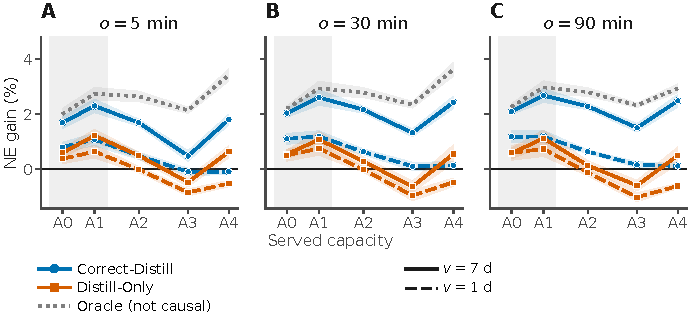
\includegraphics[width=\textwidth]{figs/gain}
\caption{$\NE$ gain over \textsc{Wait} against served capacity, one panel per join delay. Above
the line beats the conventional per-objective pipeline. Colour denotes the target and dash
denotes the attribution window, with \textsc{Oracle} drawn at $v=7$\,d to bound the panel. Bars
give the standard deviation of the per-seed differences.}
\label{fig:gain}
\end{figure}

\paragraph{A short join delay beats waiting, and by more on slow funnels.}
Writing the record \ratioSeven{} times sooner than the seven-day window it answers to, and
letting the teacher stand in for the conversions not yet seen, reduces $\NE$ in all \nCells{}
seven-day cells, of which \cdSevenSig{} survive Holm--Bonferroni correction. The reduction
ranges from \cdSevenMinAbs{}\% to \cdSevenMaxAbs{}\%, with a mean of \cdSevenMeanAbs{}\%. At the
one-day window the same substitution gains \cdOneMeanAbs{}\% on average, positive in
\cdOnePos{} of \nCells{} cells and significant in \cdOneSig{}. The two windows differ by a factor
of three, and the direction is the informative part. The slower the funnel, the more a short
join delay is worth. This inverts the natural expectation, since a longer window censors more of
the label and leaves the teacher more to supply. What dominates instead is the cost of the
alternative: \textsc{Wait} at $v=7$\,d trains on week-old data, and no amount of label accuracy
compensates for that. Both ends of the achievable interval are measured. \textsc{Oracle}, which
writes at $o$ but labels the record $\Yv$, gains \oracleSevenAbs{}\% and \oracleOneAbs{}\%, so
\textsc{Correct-Distill} recovers \recoverSeven{}\% and \recoverOne{}\% of what any causal
correction could attain. \textsc{Fresh}, the same early write with no correction at all, loses
\freshSevenAbs{}\% and \freshOneAbs{}\%. The deficit the teacher fills is an order of magnitude
larger than the gains above it.

\paragraph{The record must keep part of its hard label.}
The result above uses the hybrid target of Eq.~\eqref{eq:hybrid}. The fully soft target decides
how far it can be pushed. At $v=1$\,d, \textsc{Distill-Only} beats \textsc{Wait} by
\doOneSmallAbs{}\% at the two smallest capacities and loses to it by \doOneLargeAbs{}\% at the
three largest, crossing over between A1 and A2 at every join delay as Fig.~\ref{fig:gain} shows.
A purely soft target plausibly acts as a regulariser, supplying a variance reduction that a
small model can use and a larger one no longer needs~\cite{menon2021statistical}. The practical
consequence cuts against convenience: a record carrying no hard label is the most portable
object a consolidated pipeline could ask for, and it is exactly the one that fails at the
capacities worth serving. At $v=7$\,d the crossover is weaker and non-monotone, averaging
\doSevenLargeAbs{}\% across the three largest rungs, so we state the rule for the one-day window
and do not extrapolate it. \textsc{Correct-Distill} beats \textsc{Distill-Only} in all
\cdBeatDo{} cells, and \textsc{Wait} in \cdBeatWait{} of \nCellsBoth{}. The \cdNegN{} exceptions
both occur at $v=1$\,d and $o=5$ minutes, at rungs \cdNegWhere{}, the worse by
\cdNegWorstAbs{}\%, and neither survives correction. Their location is coherent rather than
random: the shortest join delay at the fast window is where the teacher has least to add, since
\foOneFive{} of the conversions are already visible.

\paragraph{Comparison with published methods.}
Table~\ref{tab:baselines} reports how the screened methods perform, rather than only whether
they comply.

\begin{table}[t]
\centering
\caption{Mean $\NE$ gain over \textsc{Wait} in percent, across the \nCells{} cells of each
window.}
\label{tab:baselines}
\begin{tabular}{@{}lcrr@{}}
\toprule
Method & Single-visit & $v{=}1$\,d & $v{=}7$\,d \\
\midrule
\textsc{DEFUSE} & no & +0.75 & +2.23 \\
\textsc{Fsiw}~\cite{yasui2020feedback} & yes & -0.45 & +0.31 \\
\textsc{Twice} & yes & -28.89 & -29.71 \\
\textsc{Ulc}~\cite{wang2023unbiased} & yes & +0.56 & +1.84 \\
\textbf{\textsc{Correct-Distill} (ours)} & \textbf{yes} & \textbf{+0.57} & \textbf{+1.97} \\
\bottomrule
\end{tabular}

\end{table}

Two conclusions follow. First, the one-record rule is inexpensive. Only \textsc{\bestNonSeven}
outperforms our method, and it writes \vanillaDup{} records per click to do so, buying
\priceSeven{}\,pp at seven days and \priceOne{}\,pp at one. Second, among methods that can
actually run on such a stream, ours is the strongest. \textsc{Ulc}~\cite{wang2023unbiased}
shares Eq.~\eqref{eq:hybrid} and differs only in how the corrector is estimated; we lead it by
\ourUlcSeven{}\,pp at seven days, winning \ourUlcWinSeven{} of \nCells{} cells, and match it at
one day, winning \ourUlcWinOne{} of \nCells{}. The case for an offline teacher over an online
corrector is therefore architectural rather than one of accuracy, as
Section~\ref{sec:conclusion} argues. \textsc{Twice} does not reproduce competitively under our
protocol. We report it for completeness and make no claim about its published standing; its
mechanism behaves as described, but the floor it is read against sits well above every other
method's in our harness.

\paragraph{The teacher need not be large, costly or retrained.}
Table~\ref{tab:baselines} uses the large teacher. Substituting the small one changes little.
\textsc{Correct-Distill} gains \tchSmallCdSevenAbs{}\% with the small teacher against
\tchLargeCdSevenAbs{}\% with the large one at seven days, and \tchSmallCdOneAbs{}\% against
\tchLargeCdOneAbs{}\% at one. Averaged over all \nCellsBoth{} cells the large teacher moves the
result by \teachCdMean{}\,pp for \textsc{Correct-Distill} and \teachDoMean{}\,pp for
\textsc{Distill-Only}. A \teacherRatio{}-fold increase in teacher parameters and a
\teacherFlopRatio{}-fold increase in teacher compute therefore buy nothing measurable, and the
smaller teacher is if anything marginally ahead. Holding parameters fixed while spending
\wideFlopRatio{} times more teacher compute is equally inert. The teacher's learning rate is
verified rather than inherited: the default beats a rate ten times smaller in every cell tested
and matches one twice as large, so the null result reflects a saturated teacher rather than an
untuned one. Finally, fixing the teacher after causal initialisation, so that it is shipped as a
static model rather than maintained as a second training job, costs \frzCostOneAbs{} and
\frzCostSevenAbs{}\,pp. The fixed-teacher arm still beats \textsc{Wait} in \frzBeat{} of
\frzN{} cells. Adoption therefore does not require standing up a continuously retrained
auxiliary alongside the served model.
